Bell function for a Bell basis with extra phase factor.

\begin{parts}
	\part To produce an entangled polarisation pair, we exploit the non-linear optics in BBO crystal to generate a pair of down-converted photons travelling along $\theta$ from the optic axis such that the conservation of energy and momentum are satisfied.
	\begin{figure}[H]
		\centering
		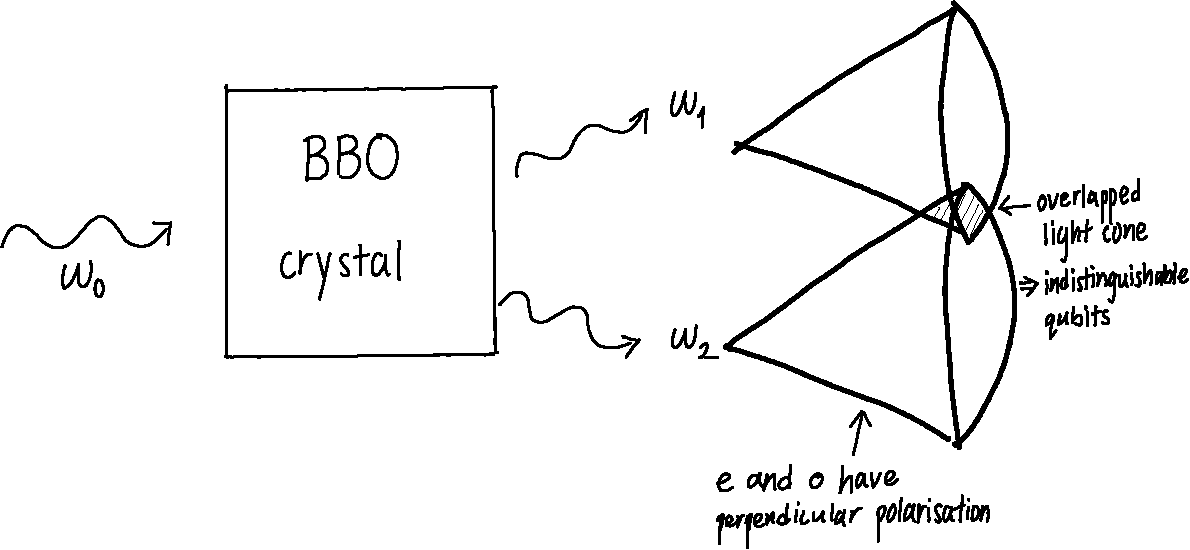
\includegraphics[width=.8\linewidth]{q6-entangled-pair}
	\end{figure}
	
	\part Starting from the given state:
	\begin{align*}
		\ket{\psi^\varphi} &= \frac{1}{\sqrt{2}} \rbracket{\ket{01} + \mathrm{e}^{i\varphi}\ket{10}} \\
		&\Rightarrow \bordermatrix{& 
			\bra{0_\textnormal{A}1_\textnormal{B}} & \bra{0_\textnormal{A}1_\textnormal{B}} & \bra{1_\textnormal{A}0_\textnormal{B}} & \bra{1_\textnormal{A}1_\textnormal{B}} \cr
			& 0 & 0 & 0 & 0 \cr
			& 0 & \dfrac{1}{2} & \dfrac{1}{2}\mathrm{e}^{i\varphi} & 0 \cr
			& 0 & \dfrac{1}{2}\mathrm{e}^{-i\varphi} & \dfrac{1}{2} & 0 \cr
			& 0 & 0 & 0 & 0 \cr
		} &= \rho_\textnormal{sys} \mtext{the system density matrix}
	\end{align*}
	
	On Alice's side, she would observe:
	\begin{align*}
		\rho_\textnormal{A} &= \textnormal{tr}_\textnormal{B} \rho_\textnormal{sys} \\
		&= \begin{pmatrix}
			\textnormal{tr} \begin{pmatrix}
				0 & 0 \\
				0 & \dfrac{1}{2}
			\end{pmatrix} &
			\textnormal{tr} \begin{pmatrix}
				0 & 0 \\
				\dfrac{1}{2}\mathrm{e}^{i\varphi} & 0
			\end{pmatrix} \\[1em]
			\textnormal{tr} \begin{pmatrix}
				0 & \dfrac{1}{2}\mathrm{e}^{-i\varphi} \\
				0 & 0
			\end{pmatrix} &
			\textnormal{tr} \begin{pmatrix}
				\dfrac{1}{2} & 0 \\
				0 & 0
			\end{pmatrix}
		\end{pmatrix} \\
		&= \begin{pmatrix}
			\dfrac{1}{2} & 0 \\
			0 & \dfrac{1}{2}
		\end{pmatrix} = \rho_\textnormal{B} \mtext{by symmetry}
	\end{align*}
	
	Note that $\textnormal{tr}(\rho_\textnormal{A}^2) = \textnormal{tr}(\rho_\textnormal{B}^2) = \diagfrac{1}{2} \neq 1$ and this indicates that we have an entangled state since each subsystem is not pure $\Rightarrow$ system is not separable.
	
	\begin{figure}[H]
		\centering
		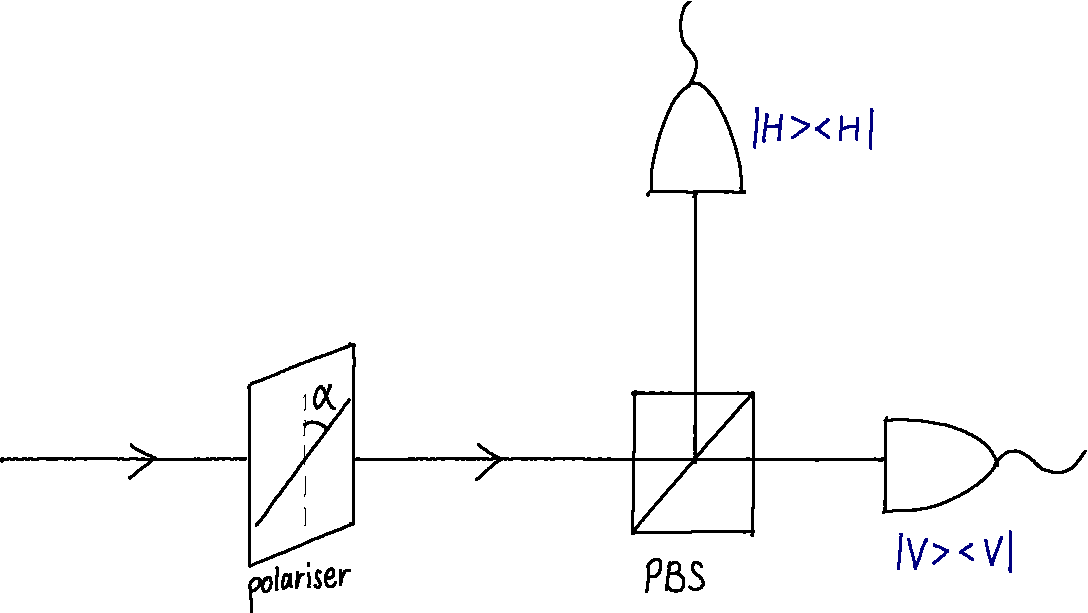
\includegraphics[width=.8\linewidth]{q6-setup}
	\end{figure}
	By setting up the chain above, one may perform a measurement of $\sigma_\alpha = \cos\alpha\,\sigma_z + \sin\alpha\,\sigma_x$.
	Alternatively, putting the PBS at an angle $\alpha$ to the vertical will achieve the same.
	
	Calculation of the expectation value:
	\begin{align*}
		\avg{\sigma_\alpha \sigma_\beta} &= \bra{\psi^\varphi} \sigma_\alpha \sigma_\beta \ket{\psi^\varphi} \\
		&= \begin{pmatrix}
			0 & \dfrac{1}{\sqrt{2}} & \dfrac{1}{\sqrt{2}} \mathrm{e}^{-i\varphi} & 0
		\end{pmatrix} \cdot \\
		&\phantom{=} \;
		\begin{pmatrix}
			\cos\alpha \begin{pmatrix}
				\cos\beta & \sin\beta \\ \sin\beta & -\cos\beta
			\end{pmatrix}
			& \sin\alpha \begin{pmatrix}
				\cos\beta & \sin\beta \\ \sin\beta & -\cos\beta
			\end{pmatrix} \\[1em]
			\sin\alpha \begin{pmatrix}
				\cos\beta & \sin\beta \\ \sin\beta & -\cos\beta
			\end{pmatrix}
			& -\cos\alpha \begin{pmatrix}
				\cos\beta & \sin\beta \\ \sin\beta & -\cos\beta
			\end{pmatrix}
		\end{pmatrix}
		\begin{pmatrix}
			0 \\ \dfrac{1}{\sqrt{2}} \\[1em] \dfrac{1}{\sqrt{2}} \mathrm{e}^{i\varphi} \\ 0
		\end{pmatrix} \\
		&= \begin{pmatrix}
			0 & \dfrac{1}{\sqrt{2}} & \dfrac{1}{\sqrt{2}} \mathrm{e}^{-i\varphi} & 0
		\end{pmatrix}
		\frac{1}{\sqrt{2}}
		\begin{pmatrix}
			\cos\alpha \sin\beta + \mathrm{e}^{i\varphi} \sin\alpha \cos\beta \\
			-\cos\alpha \cos\beta + \mathrm{e}^{i\varphi} \sin\alpha \sin\beta \\
			\sin\alpha \sin\beta - \mathrm{e}^{i\varphi} \cos\alpha \cos\beta \\
			\sin\alpha \cos\beta + \mathrm{e}^{i\varphi} \cos\alpha \sin\beta
		\end{pmatrix} \\
		&= \frac{1}{2} \sbracket{-\cos\alpha \cos\beta + \mathrm{e}^{i\varphi} \sin\alpha \sin\beta + \mathrm{e}^{-i\varphi} \sin\alpha \sin\beta - \cos\alpha \cos\beta} \\
		&= -\cos\alpha \cos\beta + \cos\varphi \sin\alpha \sin\beta
	\end{align*}
	
	We have Bell function given as: $B = \avg{QS} - \avg{RS} - \avg{RT} - \avg{QT}$.
	
	Next we make identifications $Q \equiv \sigma_0$, $R \equiv \sigma_{\pi/2}$, $S \equiv \sigma_{-3\pi/4}$, $T \equiv \sigma_{-\pi/4}$.
	
	Suppose $Q$, $R$, $S$, $T$ are related by local realism, then each random variable should be independent of one another $\Rightarrow \avg{AB} = \avg{A} \avg{B}$.
	
	Now we know each individual measurement has a possible value of $\pm 1$, so upon perfect correlation we should have $B = 1-1-1-1 = -2$.
	And similarly $B = -1+1+1+1 = +2$ for anti-correlation.
	So $|B| \leq 2$ is mandated by local realism.
	
	Now let's calculate them via QM:
	\begin{align*}
		\avg{QS} &= \avg{\sigma_0 \, \sigma_{-3\pi/4}} \\
		&= -\cos 0 \cos \rbracket{-\frac{3\pi}{4}} + \cos\varphi \sin 0 \sin \rbracket{-\frac{3\pi}{4}} \\
		&= -\cos\rbracket{-\frac{3\pi}{4}} = \frac{1}{\sqrt{2}} \\[1em]
		%
		\avg{RS} &= \avg{\sigma_{\pi/2} \, \sigma_{-3\pi/4}} \\
		&= \cos\varphi \sin\frac{\pi}{2} \sin\rbracket{-\frac{3\pi}{4}} = -\frac{1}{\sqrt{2}} \cos\varphi \\[1em]
		%
		\avg{RT} &= \avg{\sigma_{\pi/2} \, \sigma_{-\pi/4}} \\
		&= \cos\varphi \sin\rbracket{-\frac{\pi}{4}} = -\frac{1}{\sqrt{2}} \cos\varphi \\[1em]
		%
		\avg{QT} &= \avg{\sigma_{0} \, \sigma_{-\pi/4}} \\
		&= -\cos\rbracket{-\frac{\pi}{4}} = -\frac{1}{\sqrt{2}} \\[2em]
		%
		\Rightarrow B &= \frac{1}{\sqrt{2}} \rbracket{1 + \cos\varphi + \cos\varphi + 1} \\
		&= \sqrt{2} \rbracket{1 + \cos\varphi}
	\end{align*}
	
	Note that for $\sin^2 (\varphi/2) \ge 1/\sqrt{2}$, $|B| \ge 2$ and thus local realism is violated.
	
	Maximal violation when $\varphi = \pi \Rightarrow B = \sqrt{2}(1+1) = 2\sqrt{2}$.
	
	\part Average of $B$ over $\sbracket{-\varphi_0,\, \varphi_0}$:
	\begin{align*}
		\avg{B} &= \frac{1}{2\varphi_0} \int_{-\varphi_0}^{\varphi_0} \sqrt{2} \rbracket{\cos\varphi + 1} \inftsml{\varphi} \\
		&= \frac{1}{\sqrt{2}\varphi_0} \sbracket{\sin\varphi + \varphi}_{-\varphi_0}^{\varphi_0} \\
		&= \frac{\sqrt{2}}{\varphi_0} \rbracket{\sin\varphi_0 + \varphi_0} \\
		&= \sqrt{2} \rbracket{\textnormal{sinc}\,\varphi_0 + 1}
	\end{align*}
	
	This method works since we are finding $B$ for an uniform ensemble of entangled pairs with no correlation between each pair.
	
	For local realism to be violated, we need:
	\begin{gather*}
		\abs{\textnormal{sinc}\,\varphi_0 + 1} > \sqrt{2} \\
		\Rightarrow \textnormal{sinc}\,\varphi_0 > \sqrt{2} - 1 = 0.414
	\end{gather*}
	
	From the graph, we have such $\varphi_0 \approx \SI{2.1}{\radian}$ as the max value beyond which $B_{\varphi_0} < 2 \Rightarrow$ local realism holds.
\end{parts}